%!TEX  root = main.tex
\chapter{Motivations et problématique}
\label{ch:problematique}

\PartialToc

\section{Contexte industriel}

\subsection{Qu'est ce qu'un Smart Grid ?}

Le terme «~Smart Grid~» est une appellation générale désignant les technologies 
«~intelligentes~» qui «~augmentent~»\footnote{À la manière de «~l'augmentation 
de l'humain~» qui désigne l'amélioration technique des performances humaines, 
aussi bien physiques, intellectuelles qu'émotionnelles \cite{le2013humain}.} 
les réseaux électriques actuels en améliorant leurs performances. 

Cette «~augmentation~» peut servir différents objectifs dépendant des limites du 
système électrique existant, du cadre de régulation, ainsi que de 
l'orientation politique des états. Il existe autant de définitions du terme 
«~Smart Grid~» que d'objectifs motivant son implémentation. 

En Europe, les exigences de régulation et les volontés politiques des états 
membres en matière d'écologie favorisent l'intégration des énergies 
renouvelables et la participation active des consommateurs. Les Smart Grids 
européens sont donc synonymes de producteurs d'énergie renouvelables et de 
compteurs intelligents. Pour l'\gls{etp}, les Smart Grids sont ainsi «~des 
réseaux électriques qui intègrent de manière intelligente les comportements et 
les actions de tous les acteurs connectés — les producteurs, les consommateurs 
et ceux qui consomment et produisent en même temps — pour garantir une 
fourniture d'électricité efficiente, durable, économique et sûre.~» \cite{ETP}.

Les Smart Grids américains mettent, quant à eux, l'accent sur la modernisation 
des réseaux de transport d'énergie souvent très mal entretenus. Les États Unis 
doivent en effet faire face un nombre de coupures de courant qui ne cesse 
d'augmenter, passant de 76 pannes en 2007 à plus de 300 en 2011 \cite{detroit}. 
Ces pannes sont aussi fréquentes qu'importantes. En 2003, un \textit{blackout} 
dans l'Ohio prive 50 millions de personnes d'électricité et coûte 6 milliards 
de dollars \cite{andersson2005causes}. Ces coupures sont dues à la combinaison 
de trois facteurs \cite{outages}:

\begin{itemize}
    \item une infrastructure électrique vieillissante, en grande partie
    mécanisée et souffrant du manque d'investissement~;
    \item une forte croissance démographique~;
    \item des conditions climatiques de plus en plus extrêmes.
\end{itemize}

Aux États Unis, moderniser le réseau électrique en investissant dans les Smart 
Grids est ainsi essentiellement guidé par un impératif de fiabilité. Pour 
définir les Smart Grids, le département de l'énergie américain (\textit{United 
States Department of Energy}) dresse une liste d'exigences mettant en avant la 
sûreté des réseaux électriques \cite{USDE}. Selon cette définition, un Smart Grid 
doit ainsi répondre aux exigences suivantes~:

\begin{itemize}
    \item auto-réparation en cas d'événements perturbateurs~;
    \item permettre la participation active des consommateurs~; 
    \item résilience face aux attaques physiques et cybernétiques~;
    \item fournir une électricité de qualité face aux besoins du 21\up{ème}
          siècle~;
    \item intégration de moyens de production et de stockage d'électricité~;
    \item exploitation optimisée des infrastructures et conduite efficace des 
réseaux électriques.
\end{itemize} 

À partir de ces deux définitions, nous constatons que l'obsolescence du système 
électrique (dans le cas des États Unis) et les impératifs régulatoires et 
écologiques (dans le cas de l'Europe) font de la mise à niveau des réseaux 
électriques un enjeu crucial. Cette mise à niveau passe d'abord par le 
déploiement des \gls{tic} et donc par l'implémentation des Smart Grids, plutôt 
que par le remplacement massif des infrastructures électriques existantes. 

Envisager uniquement le renforcement et de remplacement massif des 
infrastructures électriques du  réseau 
n'est en effet pas une solution optimale et semble difficilement réalisable 
compte tenu de la croissance démographique constante des zones urbaines et du 
coût important des investissements à consentir \cite{cre}.

\subsection{Contexte économique, cadre législatif et \\
modes de consommation en constante mutation}

Le système électrique actuel est mis à l'épreuve par l'entrée en jeu de nouveaux 
acteurs économiques et de nouveaux cadres législatifs. 

D'une part, la libéralisation du marché de l'électricité permet à un producteur 
quelconque de produire et de vendre son électricité après s'être convenablement 
raccordé au réseau électrique de distribution ou de transport (donc entre les 
centrales de production et les consommateurs). Contrairement aux centrales de 
production localisées en amont du réseau électrique de transport, ces sources 
d'énergie sont dites distribuées. Les sources d'énergie distribuées perturbent 
fortement la stabilité des réseaux électriques. En injectant du courant, elles 
peuvent déséquilibrer le niveau de tension du réseau, endommageant ainsi les 
équipements du système électrique tels que les transformateurs, les lignes et 
les protections. 

D'autre part, les enjeux environnementaux encouragent le recours aux énergies 
renouvelables. Dans sa directive du 23 avril 2009, la commission européenne fixe 
à 20\% la part de contribution des ressources renouvelables dans la production 
totale d'énergie à l'horizon de 2020. Les réseaux électriques sont de ce fait 
amenés à connaître une croissance constante de ces producteurs décentralisés 
dans les années à venir.

Cette même directive fixe à 20\% la réduction des émissions de gaz à effet de 
serre par rapport à leur niveau en 1990 et à 20\% l'augmentation de l'efficacité 
énergétique. Or les pics de consommation en période de pointe sont coûteux et 
émetteurs de CO\textsubscript{2}. Ces pics apparaissent typiquement en fin de journée d'un 
jour de semaine lorsque les gens allument leurs télévisions, plaques électriques 
et autres outils électroménagers en rentrant chez eux.  En effet, pour maintenir 
l'équilibre entre l'offre et la demande d'électricité en cas de pics de 
consommation, les producteurs recourent à des centrales à charbon, à fioul et à 
gaz comme l'illustre la figure~\ref{fig:courbeCharge}.


\begin{figure}[!htbp]
 \begin{center}
  
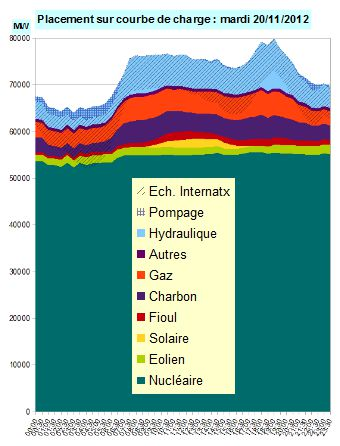
\includegraphics[width=0.5\textwidth]{figures/1_problematique/ccharge.jpg}
 \end{center}
 \caption{Placement du type d'énergie sollicitée sur la courbe de charge 
française du mardi 20 novembre 2012 (à remplacer par une plus 
belle/récente)(source RTE)}
 \label{fig:courbeCharge}
\end{figure}

Ces pics s'intensifient significativement avec l'émergence de nouveaux usages de 
consommation d'énergie dont, notamment, la mobilité électrique. En France, les 
pouvoirs publics estiment à deux millions le nombre de véhicules électriques en 
circulation en 2020. L'impact de ces véhicules sur l'équilibre entre l'offre et 
la demande n'est pas négligeable. En effet, la recharge complète d'un véhicule 
électrique ayant 150 km d'autonomie est équivalente en termes d'appel de 
puissance à~:
\begin{itemize}[noitemsep]
    \item un chauffe-eau si la recharge s'effectue en 8~h (recharge normale)~;
    \item un immeuble si la recharge s'effectue en 1~h (recharge accélérée)~;
    \item un quartier urbain si la recharge s'effectue en 3~min (recharge rapide).
\end{itemize}



\subsection{Architecture des Smart Grids : \\
vers des réseaux électriques flexibles et communicants}

Pour faire face aux mutations du contexte énergétique, les gestionnaires de 
réseaux électriques ne peuvent plus compter uniquement sur la conduite 
prévisionnelle du réseau électrique (peu réactive face à l'intermittence des 
énergies renouvelables par exemple) ni envisager le redimensionnement du réseau 
(onéreux et non optimal). 

La solution réside dans l'automatisation de la conduite des réseaux électriques, 
grâce a l'acquisition et l'exploitation en temps réel d'informations sur l'état 
des réseaux. Cela passe par le déploiement d'un réseau informatique au niveau 
des infrastructures électriques, et la mise en place dans le \gls{si} d'outils 
pour l'exploiter.

Ainsi équipés, les réseaux électriques s'apparentent à une toile d'araignée où 
les mailles interagissent constamment via des liens de communication. Ces 
mailles correspondent aux acteurs du système électrique~: consommateurs, 
producteurs ou les deux à la fois. Outre l'électricité, ces acteurs produisent 
et consomment de l'information en temps réel grâce aux modules logiciels dont 
ils sont équipés et à divers moyens de télécommunication, tels que les réseaux 
mobiles ou le \gls{cpl}. Ce partage permanent et 
instantané d'informations entre les équipements préserve la stabilité du 
système électrique tout en augmentant son efficacité énergétique.

Pour illustrer les possibilités offertes par les \gls{tic}, prenons l'exemple 
du pic de consommation de la fin de journée d'un jour en semaine. Grâce aux 
\gls{tic}, il devient possible d'agir sur la demande plutôt que sur l'offre. Le
distributeur d'électricité, s'appuyant sur des points de contrôle distants et 
des compteurs intelligents installés chez les clients pour envoyer et recevoir 
des informations et des consignes, peut alors adresser des demandes 
d'effacement aux consommateurs moyennant des incitations tarifaires. Il peut 
s'agir d'une coupure du chauffage pendant 15~min à 30~min d'un foyer ou d'un 
bureau bien isolé. Sans incidence sur le confort des consommateurs, ces 
demandes d'effacement aident à lisser la courbe de charge aux heures de pointe 
tout en évitant de mobiliser des centrales de production. 

Nés de la convergence des réseaux électriques et des \gls{tic}, les Smart Grids 
se composent de trois couches que nous retrouvons dans la figure~\ref{fig:archismartGrids}~:

\begin{enumerate}
    \item le premier niveau correspond à l'infrastructure et aux équipements 
    électriques acheminant l'électricité tels que les lignes et les 
    transformateurs~; 
    \item le second niveau correspond à l'infrastructure de communication 
    composée de différentes technologies de télécommunication comme la fibre 
    optique, le \gls{cpl}, ou encore la \gls{3g}~; 
    \item le troisième niveau correspond aux applications informatiques qui 
    incarnent «~l'intelligence~» du réseau. En utilisant des informations 
    délivrées en temps réel, ces applications calculent des consignes à envoyer 
    aux équipements concernés et automatisent ainsi la conduite du système 
    électrique.  Cette intelligence est centralisée au niveau des centres de 
    conduite du réseau ou distribuée sur les équipements électriques. 
\end{enumerate}

\begin{figure}[!htbp]
  
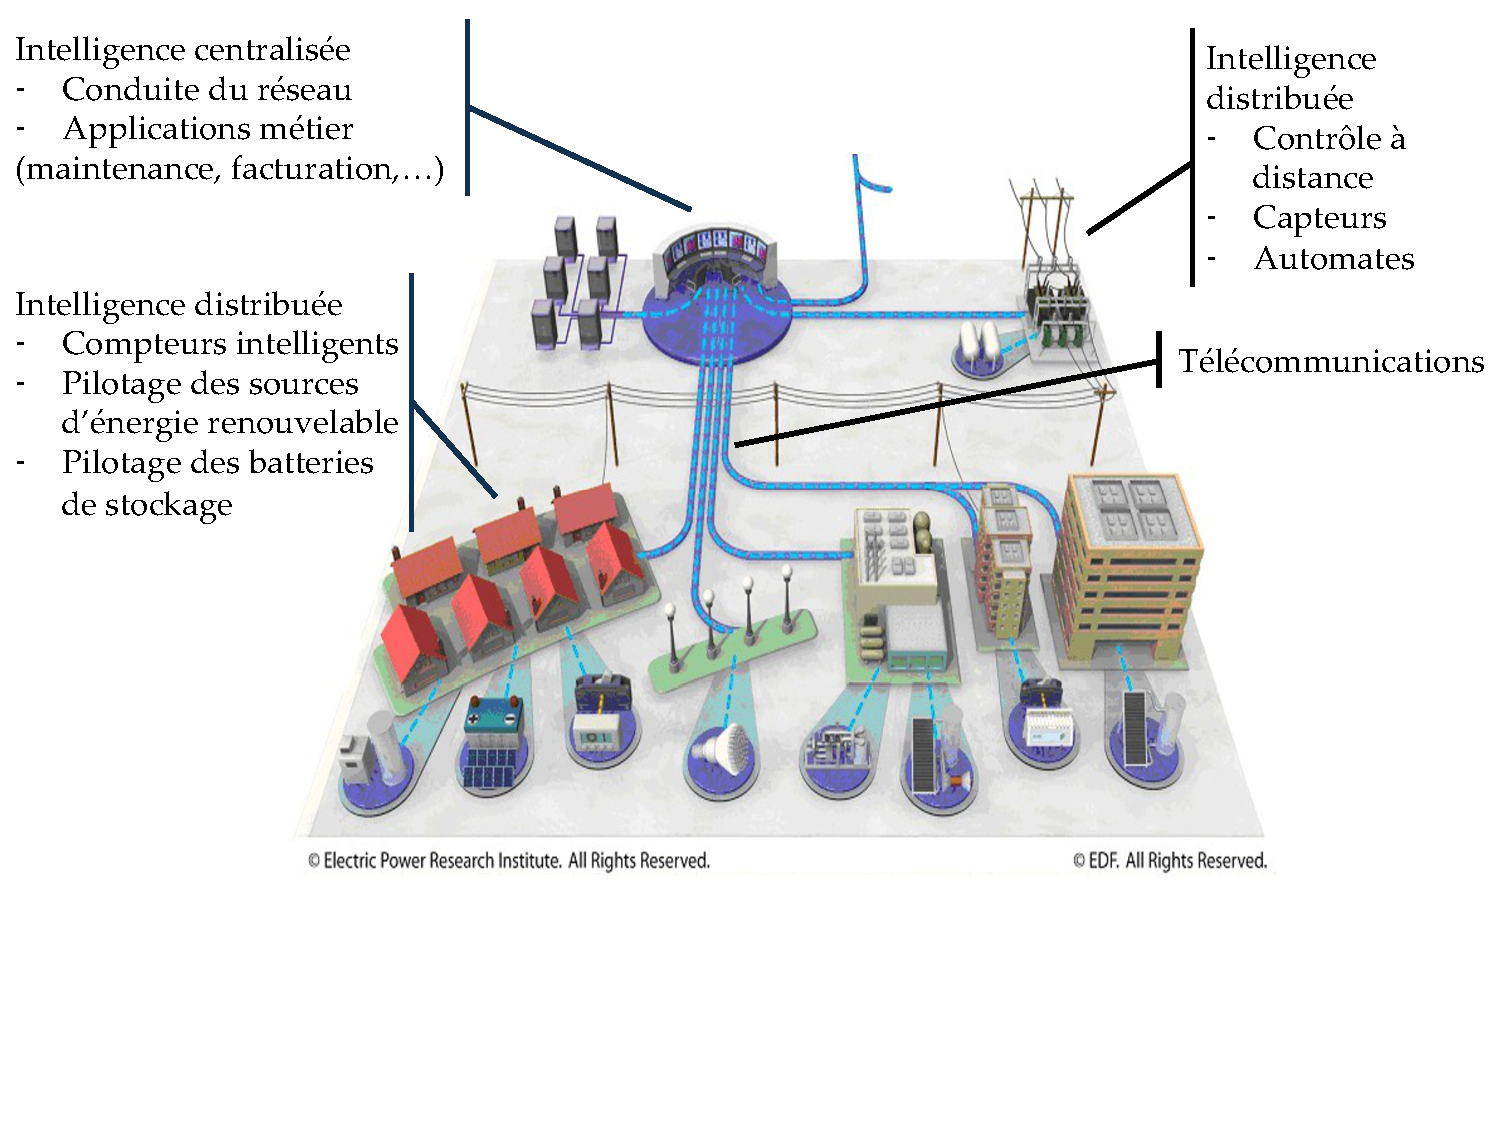
\includegraphics[trim= 0cm 4cm 0cm 0cm, width=1\textwidth]{figures/1_problematique/archiSmartGrids.pdf}
 \caption{Architecture des Smart Grids \protect\cite{favre2006ingenierie}}
 \label{fig:archismartGrids}
\end{figure}


%En effet, la libéralisation du marché de l'électricité exige que le 
%consommateur ait une connaissance en temps réel de l'évolution tarifaire 
%horaire 
%de l'électricité et qu'il puisse même choisir d'injecter sa propre propre 
%production d'énergie sur le réseau.

\section{Problématique industrielle}
%la nécessaire évolution des Systèmes d'Information pour la mise en œuvre d'une stratégie orientée Smart Grids

%Un Smart Grid est un réseau électrique intelligent permettant d'optimiser la 
%production, la distribution et la consommation d'électricité grâce à 
%l'introduction des Technologies de l'Information et de la Communication (TIC) 
%sur le réseau électrique \footnote{www.smartGrids-cre.fr}.

En traitant les données envoyées en temps réel par les capteurs installés sur 
les équipements électriques et chez les consommateurs, les \gls{si} calculent 
des consignes destinées à des organes télécommandés permettant ainsi de piloter 
les 
réseaux électriques à distance. 
Cette automatisation de la gestion des réseaux est une solution pour les adapter 
rapidement face aux contraintes qu'introduit l'intégration des énergies 
renouvelables et des nouveaux usages \cite{cre}. Les \gls{si} sont donc au cœur 
des 
enjeux Smart Grids.  

L'implémentation des Smart Grids va ainsi de pair avec la mise à niveau des 
\gls{si} des gestionnaires du réseau électrique. En effet, ces \gls{si} doivent 
pleinement intégrer les évolutions qu'induisent les Smart Grids au niveau des 
processus 
métier du gestionnaire de réseau, des acteurs impactés, des informations 
échangées ainsi que des applications informatiques et des infrastructures 
techniques sous-jacentes. Parmi ces évolutions nous citons~:

\begin{itemize}
    \item les nouveaux flux d'information provenant du réseau électrique~;

    \item l'entrée en jeu de nouveaux acteurs tels que les producteurs
    décentralisés (éolien, photovoltaïque)~;

    \item les nouveaux équipements communicants comme le compteur Linky 
(\gls{erdf} 
    annonce le déploiement de 30 millions de compteurs d'ici 
    2020\footnote{www.erdf.fr/Linky})~;

    \item les nouvelles réglementations et directives européennes (dans le cas 
    des gestionnaires de réseaux européens)~;

    \item les nouveaux usages comme les véhicules électriques ou encore les 
    maisons connectées.
\end{itemize}

Outre leurs \gls{si}, les gestionnaires de réseaux électriques doivent faire 
évoluer 
leurs stratégies de développement en envisageant de nouveaux modèles métier et 
de nouveaux partenaires, tout en tenant compte de l'émergence des nouvelles 
technologies et des exigences du législateur. Une étude américaine, menée par 
IBM, CISCO, EPRI et South Carolina Edison, fait état de cinq thèmes stratégiques 
clés pour l'implémentation des Smart Grids~:

\begin{itemize}

    \item \textbf{permettre au consommateur de contrôler sa consommation 
    d'énergie} et de réduire son empreinte carbone en utilisant des équipements 
    intelligents et des véhicules électriques et en produisant de l'énergie 
    renouvelable à domicile~;

    \item \textbf{améliorer la sécurité et la productivité des employés} en 
    mettant par exemple à leur disposition des outils performants pour le 
    contrôle à distance, des équipements de protection, et des applications 
    mobiles~; 

    \item \textbf{intégrer des sources d'énergie renouvelables} distribuées sur 
    le réseau en assurant la protection des équipements électriques, le 
    stockage de l'énergie et la stabilité du réseau~; 

    \item \textbf{améliorer l'efficience et la résilience du réseau} à travers 
    les systèmes de mesure en temps réel, l'analyse et le contrôle à distance~;

    \item \textbf{fournir les informations et la connectivité nécessaires} en
    developpant une infrastructure \gls{tic} pour répondre aux besoins 
    d'informatisation du réseau électrique. Ce dernier point est une condition 
    \textit{sine qua non} de la réalisation des quatre précédents.
\end{itemize}

Compte tenu de ces thèmes clés, les gestionnaires de réseaux envisagent des 
stratégies impliquant l'adoption de technologies Smart Grids. 
La mise en œuvre effective de ces stratégies demande l'automatisation des 
actions sur le réseau et du traitement des données, ce qui entraine donc le 
déploiement de nouveaux \gls{si}. Afin d'appréhender ces paradigmes naissants, 
des 
scénarios métier sont élaborés mais il est indispensable de les éprouver et de 
les valider avant d'envisager leur implémentation finale.

Plusieurs démonstrateurs physiques ont été déployés sur le terrain 
\footnote{www.erdf.fr/Carte\_demonstrateurs\_Smart\_Grids}. Ces projets pilotes 
permettent de mener des expérimentations en conditions réelles pour tester des 
fonctions et des services, comme par exemple le démonstrateur InfiniDrive 
\footnote{avem.fr/actualite-erdf-et-le-groupe-la-poste-lancent-le-projet-infini-drive-a-nice-3450.html} 
pour le pilotage des infrastructures de recharge de véhicules électriques ou le 
démonstrateur Venteea \footnote{www.venteea.fr} pour l'intégration d'une forte 
capacité éolienne dans un réseau rural. Cependant, les démonstrateurs 
nécessitent que le gestionnaire de réseau de distribution recrute des clients 
industriels et/ou domestiques qui acceptent d'avoir du matériel à tester chez 
eux. De plus, leur exploitation reste limitée par les réglementations en cours. 
Enfin, leur mise en place se révèle souvent longue et coûteuse. 

En plus de ces démonstrateurs, des réseaux de distribution d'expérimentation 
grandeur nature tel que Concept Grid \footnote{chercheurs.edf.com}, implanté à 
\gls{edf} Lab, permettent de tester les nouveaux équipements avant leur 
installation sur les réseaux du distributeur \gls{erdf}. Ces réseaux ont 
l'avantage de permettre la conduite de \textit{stress tests} en conditions perturbées, 
impossibles à réaliser dans le cadre de démonstrateurs, ceux-ci impliquant de 
vrais clients. Cependant, la taille réduite de ces réseaux reste limitante. 

Pour pallier toutes ces limitations, une troisième voie est la simulation. La 
simulation intègre les trois couches qui composent les Smart Grids~: 
l'infrastructure électrique (transformateurs, lignes, charges, sources), 
l'infrastructure de télécommunication (réseaux mobiles, \gls{cpl}) et enfin les 
\gls{si} qui 
les pilotent. Des simulateurs spécialisés dans la simulation de réseaux 
électriques (EMTP-RV, Dymola, PowerFactory, Eurostag, etc.) ainsi que des 
simulateurs de réseaux de télécommunication (OPNET, NS-3, OMNeT ++, etc.) ont 
déjà validé l'apport de la simulation dans leurs domaines respectifs. Toutefois, 
les \gls{si} sont souvent relégués à de simples modèles de calcul de consignes 
souvent 
développés en Matlab ou en C++ \cite{palensky2014simulating}. 

Dans ce contexte, la problématique industrielle dans laquelle  s'inscrivent nos 
travaux de recherche est donc la suivante~: 

\textbf{Comment valider une stratégie de développement orientée Smart Grids à 
travers la simulation de sa déclinaison au niveau du SI du gestionnaire du 
réseau électrique~?}

 
\section{Problématique de recherche}

%\subsection{Le recours à l'Architecture d'Entreprise}

Les technologies Smart Grids illustrent le défi que représente l'évolution des 
\gls{tic} et l'intégration des énergies renouvelables pour les gestionnaires de 
réseaux électriques. Jeremy Rifkin annonce même «~une troisième révolution 
industrielle, fondée sur le couplage des technologies de l’Internet et des 
énergies nouvelles~» \cite{rifkin2012troisieme}. 

Mais à l'ère numérique, l'adaptation au changement relève des préoccupations de 
toute entreprise s'appuyant sur les \gls{tic} pour mener ses 
activités. Le très haut niveau de concurrence que connait le secteur des 
technologies de l'information stimule l'innovation. Or ces technologies sont de 
plus en plus le moteur qui fait progresser les  métiers de l'entreprise. Être 
capable de s'adapter continuellement à l'évolution rapide et 
constante des \gls{tic} représente donc un véritable challenge pour les 
entreprises 
d'aujourd'hui.

Pour mener à bien tout changement, il est primordial de commencer par une 
description représentative de «~l'objet~» à changer, qu'il s'agisse d'une 
nouvelle version d'un avion, d'une voiture, d'un ordinateur ou encore d'une 
entreprise \cite{zachman1997enterprise}. Cette description représentative 
revient à concevoir l'architecture de l'objet en question. L'architecture en 
tant qu'activité est centrale dans plusieurs disciplines, allant de 
l'architecture du bâtiment à l'architecture logicielle, en ce qu'elle est un 
outil indispensable à la construction d'artefacts respectant les qualités 
attendues de l'objet final. En précurseur, Zachman \cite{zachman1997enterprise} 
recommande d'appliquer les principes d'architecture à l'entreprise pour faire 
face aux changements dictés par l'innovation technologique.

Les \gls{si} sont en première ligne dès qu'il s'agit de l'évolution des 
\gls{tic}. Nos 
travaux se sont donc d'abord portés sur l'évaluation de l'impact de cette 
évolution sur les \gls{si} de l'entreprise. De ce fait, nous nous sommes d'abord 
appliqués à décrire l'architecture de ces \gls{si} \cite{seghiri2015simulation}. 

Les changements apportés par ces technologies impactent cependant, non seulement 
les \gls{si}, mais l'entreprise dans son ensemble~: de sa stratégie à ses 
partenaires, en passant par ses objectifs, ses clients et ses processus métier. 
Par exemple, 
l'utilisation des véhicules électriques fait évoluer le \gls{si} du 
gestionnaire du réseau électrique qui doit mettre en place de nouvelles 
applications capables de bien gérer leur recharge. Mais il doit aussi faire 
évoluer son modèle métier en mettant à disposition de nouveaux contrats 
client favorisant la recharge hors de la période des pics de consommation par exemple, 
ou encore créer de nouveaux partenariats avec les constructeurs 
automobiles comme dans le cas d'\gls{edf} et Renault-Nissan qui collaborent sur 
un système de recharge pour véhicule électrique permettant à ce dernier de 
communiquer avec les bornes de recharge.

Évaluer l'adoption de nouvelles technologies de l'information oblige à prendre 
en compte l'entreprise dans son ensemble afin de garantir une cohérence entre 
la stratégie d'évolution adoptée et les \gls{si} qui implémentent cette 
stratégie. Parce que l'alignement entre la stratégie métier et le \gls{si} est 
au cœur de l'\gls{ea}\footnote{L'acronyme EA (\textit{Enterprise Architecture}) 
est souvent utilisé même dans la communauté francophone.} 
\cite{zachman1997enterprise}, nous
adoptons l'\gls{ea} pour évaluer l'impact des technologies Smart Grids sur les
gestionnaires des réseaux électriques. Il est en effet indispensable de
concevoir une architecture cible pour avoir  «~une vision générale de comment
une entreprise va mettre en œuvre sa stratégie~» \cite{ross2006enterprise}.

L'\gls{ea} participe à l'alignement des composants d'une entreprise en offrant 
une vision globale et transverse \cite{zachman1987framework}. Dans le contexte 
des 
Smart Grids par exemple, elle permet d'aligner efficacement les intérêts des 
acteurs impliqués dans leur implémentation tels que les experts métier, les 
conseillers stratégiques, les experts environnementaux ou encore les experts en 
normalisation.

L'exécution effective d'une stratégie est cependant confrontée à des barrières 
de communication au sein de l'entreprise \cite{vcater2010factors}. Le recours à 
l'\gls{ea} est d'autant plus justifié qu'elle représente un outil pour la 
transmission des objectifs stratégiques à tous les niveaux hiérarchiques de 
l'organisation en 
question \cite{kappelman2008enterprise}. 

Pour toutes ces raisons, nous souhaitons mettre à profit les principes 
d'\gls{ea} pour évaluer l'impact de l'adoption des technologies Smart Grids sur 
les \gls{si} des 
gestionnaires de réseaux électriques, tout en garantissant la cohérence entre la 
stratégie adoptée et les \gls{si} qui les implémentent. 

%\cite{buckl2010conceptual}. Le recours à l'architecture d'entreprise est ainsi 
%pleinement justifié.

%\subsection{Le recours à la simulation}

Les Smart Grids correspondent à des systèmes dynamiques et complexes 
\cite{monti_power_2010} étant donné le grand nombre de parties prenantes qui 
interagissent eux (tels que les producteurs d'énergie renouvelable ou les 
consommateurs actifs sur le réseau), tout en ayant des comportements autonomes 
et des objectifs différents. Les \gls{si} pilotant les  Smart Grids 
correspondent par conséquent à des systèmes dynamiques aux comportements 
complexes. Borshchev et 
Filippov\cite{borshchev2004system} affirment que le seul moyen d'adresser cette 
complexité est de simuler ces systèmes. La simulation est une technique connue 
pour valider ou critiquer la conception d'un système dès les premières étapes 
de son cycle de développement. Les acteurs impliqués dans le déploiement des 
Smart Grids acquièrent, par la  simulation, une connaissance approfondie et 
directe des modèles créés pour valider ou critiquer leur choix d'implémentation.

Néanmoins, les approches d'\gls{ea} se focalisent le plus souvent sur des 
aspects statiques et structurels tels que les interconnexions entre les 
différentes applications métier \cite{buckl2008towards}. De plus, les modèles 
issus de ces 
approches sont ne sont pas exécutables et sont conçus en 
priorité pour la documentation et la communication entre parties prenantes 
\cite{kulkarni2013modelling}. Notre problématique de recherche se résume de ce 
fait dans la question suivante :

\vspace*{1em}
\begin{framed}
{\bfseries Quels méthodes, modèles et outils adopter pour simuler une 
architecture d'entreprise afin de la valider?}
\end{framed}




